% !TeX encoding=utf8
% !TeX spellcheck = de-CH

\chapter{Dokumentation}
In diesem Kapitel wird der Aufbau der Implementation mit den verschiedenen Komponenten näher beschrieben.

\section{Übersicht der Struktur}
Die Sourcen, Dokumentation, etc. befinden sich in unserem Github-Repository (Siehe Kapitel \ref{sec:Projektmanagement:Tools})
\subsection{Server Seite}
Das Backend befindet sich im Repository unter \textit{/code/server} und ist in folgende Module aufgeteilt:

\begin{itemize}
\item {\textbf{Main} - dcf77\_main.c} \\
Das Main-Modul verbindet alle übrigen Module miteinander und stellt die Kommunikation untereinander sicher.

\item {\textbf{DCF77 Reader} - dcf77\_reader.c} \\
Der Reader liest die Daten von der USB-Schnittstelle zum DCF77 und übergibt diese dem Decoder.

\item {\textbf{DCF77 Decoder} - dcf77\_decoder.c}\\
Der Decoder decodiert laufend die erhaltenen Daten von der USB-Schnittstelle und generiert pro Minute einen entsprechenden Timestamp. Voraussetzung dafür ist, dass  genügend Daten empfangen wurden und keine Fehler aufgetreten sind. Der Timestamp wird anschliessend dem Clock-Modul zur Synchronisation übergeben.

\item {\textbf{Clock} - Clock.c}\\
Das Clock-Modul bildet eine eigenständige, laufende Uhr. Wird ein DCF77-Signal erfolgreich decodiert, so werden die Informationen (Datum und Zeit) sekundengenau übernommen. Anschliessend läuft die Uhr autonom weiter. Als Basis wird die Systemzeit des Server-Hosts verwendet.

%TODO Wie überprüfen wir das Signal?! -> 2 Timestamps zum Vergleich

\item {\textbf{Server} - SimpleSocketServer.c}\\
Der Server bietet eine Web-Schnittstelle via Sockets an, welche den Timestamp, gemäss ISO 8601\footnote{Spezifikation: \url{http://www.iso.org/iso/home/standards/iso8601.htm}}, als JSON anbietet. Der Timestamp wird aus der aktuellen Zeit aus dem Clock-Modul erzeugt.

\end{itemize} 

\subsection{Client Seite}
Das Frontend befindet sich im Repository unter \textit{/code/client}. Das Frontend ist eine Web-Oberfläche, welche die entsprechenden GUI-Elemente darstellt und via HTTP-Request in bestimmten Zeitintervallen die aktuelle Zeit vom Server abruft.\\

%TODO: Plugins auflisten und kurz beschreiben, Quellen angeben
Für die Darstellung haben wir folgende Plugins verwendet:
\begin{itemize}
\item \textbf{jQuery \& jQuery UI}\\
Das wohl bekannteste JS Framework, das einem in jeglichen Bereichen unterstützt und Umsetzungen vereinfacht. jQuery UI ist ein GUI für das Web, welches auf jQuery basiert. (\url{http://jquery.com/}, \url{http://jqueryui.com/} )

\item \textbf{Bootstrap}\\
Von Twitter eine Struktur-Vorlage um eine moderne Website umzusetzen. Sie bietet gängige Funktionen (Responsive, Informtionen Elements, Navigation, etc.) und grundlegende Styles an. (\url{http://getbootstrap.com/})

\item \textbf{CoolClock}\\
Die CoolClock ist ein Projekt in dem eine analoge Uhr vollständig mit HTML 5, CSS und JS umgesetzt worden ist. (\url{http://randomibis.com/coolclock/})

%\TODO Dani \item digiClock

\end{itemize}

%TODO: Screenshot`/ Screendesign?

\section{Modul-Dokumentation}
Die Funktionsweise, der einzelnen Module, wurde innerhalb des Codes dokumentiert und beschrieben. Nachfolgend werden die wichtigsten Aspekte der Umsetzung kurz erläutert.

\subsection{DCF Reader}
Source: \textit{/code/server/dcf77\_reader.c}\\
Via Schnittstelle zum "`Expert mouse CLOCK USB II"' wird der Status der Warteschlange  solange abgerufen, bis mindestens ein Wert (8-Bit Integer) bereit ist.
Sobald ein Wert vorhanden ist, wird dieser ausgelesen und direkt dem Decoder übergeben.

Da das Programm seriell abläuft, ist es wichtig, dass wir pro Verarbeitung nicht länger als eine Sekunde benötigen, denn dann muss das nächste Signal verarbeitet werden können.
Dadurch das die ganze Software in C implementiert wurde, und keine sehr aufwändigen Berechnungen durchgeführt werden müssen, stellt dies kein Problem dar.

\subsection{DCF Decoder}
Source: \textit{/code/server/dcf77\_decoder.c}\\
Der Decoder mappt jedes erhaltende Byte direkt einem Bit zu. Laufend werden aus den verfügbaren Bits, via 4 Paritäsbit, gültige Daten gesucht. Ein vollständiges Datum besteht aus 39 fortlaufenden Bits. Zur Validierung wird das Datum auf grundlegende Datum-Korrektheit überprüft. Als zusätzliche Validierung können Datum-Informationen mit der Systemzeit abgeglichen werden (diese Funktion wurde allerdings auskommentiert, da dies nicht einsatzwürdig sei).
Wird ein gültiges Datum gefunden, so wird dies direkt der Systemclock übergeben.

\subsection{Clock}
Source: \textit{/code/server/Clock.c}\\
Die Clock wird zu Beginn mit der aktuellen Systemzeit initialisiert. Anschliessend wird mit Hilfe der POSIX-Alarm Funktion jede Sekunde eine Funktion ausgeführt, welche die Zeit erhöht. Dabei werden die Standardmässigen Regeln für die Zeitzählung angewendet.
\begin{itemize}
\item 1 Minute: 60 Sekunden
\item 1 Stunde: 60 Minuten
\item 1 Tag: 24 Stunden
\item 
\begin{itemize}
\item Januar, März, Mai, Juli, August, Oktober, Dezember: 1 Monat: 31 Tage 
\item April, Juni, September, November: 1 Monat: 30 Tage
\item Februar:
\begin{itemize}
\item Aktuelles Jahr ist ein Schaltjahr: 29 Tage 
\item Aktuelles Jahr ist kein Schaltjahr: 28 Tage
\end{itemize}
\end{itemize}
\item 1 Jahr: 365 Tage (366 Tage in einem Schaltjahr)
\end{itemize}

Das Schaltjahr wird wie folgt berechnet. Grundsätzlich gilt: Ist die aktuelle Jahreszahl ohne Rest durch 4 teilbar ist dies ein Schaltjahr. Ist dasselbe Jahr jedoch auch restlos durch 100 teilbar handelt es sich trotzdem um kein Schaltjahr, ausgenommen das Jahr lässt sich restlos durch 400 teilen, dann handelt es sich wiederum um ein Schaltjahr.

Die Uhr bietet eine Funktion an, mit welchem die Zeit "`synchronisiert"' und auf einen bestimmten Wert gesetzt werden kann. Bei der Synchronisierung wird eine Plausibilisierung der zu synchronisierenden Zeit vorgenommen. Es werden dabei nachfolgende Regeln für die Überprüfung angewendet. Wir haben uns bewusst dafür entschieden die Validierung nur bis auf Stunden-Ebene zu implementieren, da je nach Empfangsqualität nur einige wenige Signale vom DCF77 empfangen werden können.

\begin{itemize}
\item Jahr: 
	\begin{itemize}
		\item Jahr entspricht aktuellem Jahr
		\item Jahr entspricht dem nächsten Jahr
			\begin{itemize}
				\item Monat entspricht dem Januar
				\item Tag entspricht dem 01.
			\end{itemize}
		\item Jahr entspricht dem letzten Jahr
			\begin{itemize}
				\item Monat entspricht dem Dezember
				\item Tag entspricht dem 31.
			\end{itemize}
	\end{itemize}
\item Monat:
	\begin{itemize}
		\item Monat entspricht aktuellem Monat
		\item Monat entspricht dem nächsten Monat
			\begin{itemize}
				\item Tag entspricht dem 01.
			\end{itemize}
		\item Monat entspricht dem letzten Monat
			\begin{itemize}
				\item Tag entspricht dem Letzten des letzten Monats.
			\end{itemize}
	\end{itemize}
\item Tag:
\begin{itemize}
	\item Tag entspricht aktuellem Tag
	\item Tag entspricht dem nächsten Tag
		\begin{itemize}
			\item Stunde entspricht 0.
		\end{itemize}
	\item Tag entspricht dem letzten Tag
		\begin{itemize}
			\item Stunde entspricht 23.
		\end{itemize}
\end{itemize}
\item Stunde:
	\begin{itemize}
		\item Stunde entspricht aktueller Stunde
		\item Stunde ist grösser gleich der vorletzten Stunde.
		\item Stunde ist kleiner gleich der übernächsten Stunde.
	\end{itemize}
\end{itemize}

Das aktuelle Jahr (Monat, Tag, Stunde) bezeichnet die aktuelle Zeit der Clock (vor der Synchronisation).

Um konkurrierende Zugriffe zu verhindern, werden Semaphoren eingesetzt.

Uns ist bewusst, dass die aktuelle Implementation der Uhr je nach Systemlast unterschiedlich stark abweichen kann. Hier mussten wir jedoch aus zeitlichen Gründen einen Kompromiss eingehen. Ursprünglich war gedacht, dass für die Bestimmung einer Sekunde der System-Tic verwendet wird. Dieser generiert 18.2 mal in der Sekunde einen  Tic-Interrupt. Die Registrierung einer entsprechenden Interrupt Service Routine oder das explizite Abfragen des Tics erfordert unter allen modernen Betriebssystemen höhere Rechte (Kernel Mode). Dafür müsste entweder ein eigener Geräte-Treiber oder ein Kernel-Modul implementiert werden. Da wir auch nach einigen Anläufen keine funktionierende Lösung realisieren konnten, haben wir uns für die Implementation der vereinfachten Variante entschieden.

\subsection{Simple Web Server}
Source: \textit{/code/server/SimpleSocketServer.c}\\
Aus dem Main-Modul heraus wird ein simpler Socket Server in einem separaten Thread gestartet. Der Server arbeitet nur auf einem Thread. Multithreading muss in C selbst implementiert werde. Dies haben wir aufgrund der Rahmenbedingungen bewusst nicht implementiert. Wird eine Verbindung zum Server hergestellt wird mit Hilfe einer Hilfs-Funktion und der Zeit aus dem Clock-Modul ein JSON-String generiert und an den Client zurückgesendet. Die Implementation des Servers wurde bewusst so minimal als möglich gehalten.

\section{System-Voraussetzungen}
Für die Ausführung gelten folgende Systemvoraussetzungen:

\begin{itemize}
\item OS: Windows oder Mac OSX (32- und 64-bit)
\item C-Programme Kompilierung und Ausführung (für Windows empfiehlt sich eine Cygwin-Installation)
\item Aktueller Browser (Chrome, Mozilla Firefox, Internet Explorer), JavaScript muss aktiviert sein
\end{itemize}

\section{Installationsanleitung - DCF77-Treiber}
\subsection{OSX}
Für das Auslesen der Daten wird der D2xx Treiber genutzt. Eine genau Anleitung zur Installation ist in folgendem Dokument in Kapitel "`3.2 Installing D2xx Drivers"' (Seite 9) beschrieben.

Im Git Repo unter:\\
\textit{/analyse/AN\_134\_FTDI\_Drivers\_Installation\_Guide\_for\_MAC\_OSX.pdf}

\subsection{Windows}
Um die Applikation unter Windows zu kompilieren, muss der Pfad zu den Treiber-Libraries dem Compiler bekannt gegeben werden. Ansonsten sind keine weiteren Schritte notwendig.

\section{Betrieb}
\subsection{Server}
Im Verzeichnis \textit{code/server} können via \textit{make} (Windows: "`\textit{make fullWin}"', OSX: "`\textit{make fullOsx}"') die ausführbaren Dateien generiert werden.

Anschliessend kann die ausführbare Datei "`./controlledClock.exe"' gestartet werden. Um das DCF77 Signal zu empfangen, muss der Empfänger korrekt installiert und angeschlossen sein. Das Programm ist aber auch ohne Empfänger ausführbar, und kann für die Synchronisation verwendet werden.

\subsection{Client}
Der Client ist komplett in HTML, JS und CSS geschrieben und kann deshalb ohne Installation ausgeführt werden. 

Um den Client zu starten, muss die Datei "`index.html"' im Client-Verzeichnis geöffnet werden. Um eine Synchronisation auszuführen, muss der Server laufen.

\newpage
\section{Screenshots}

\subsection{Server}

\begin{figure}[htbp!]
	\caption{Konsolen Output bei laufendem Server (mit DCF77 via USB)}
	\centering
		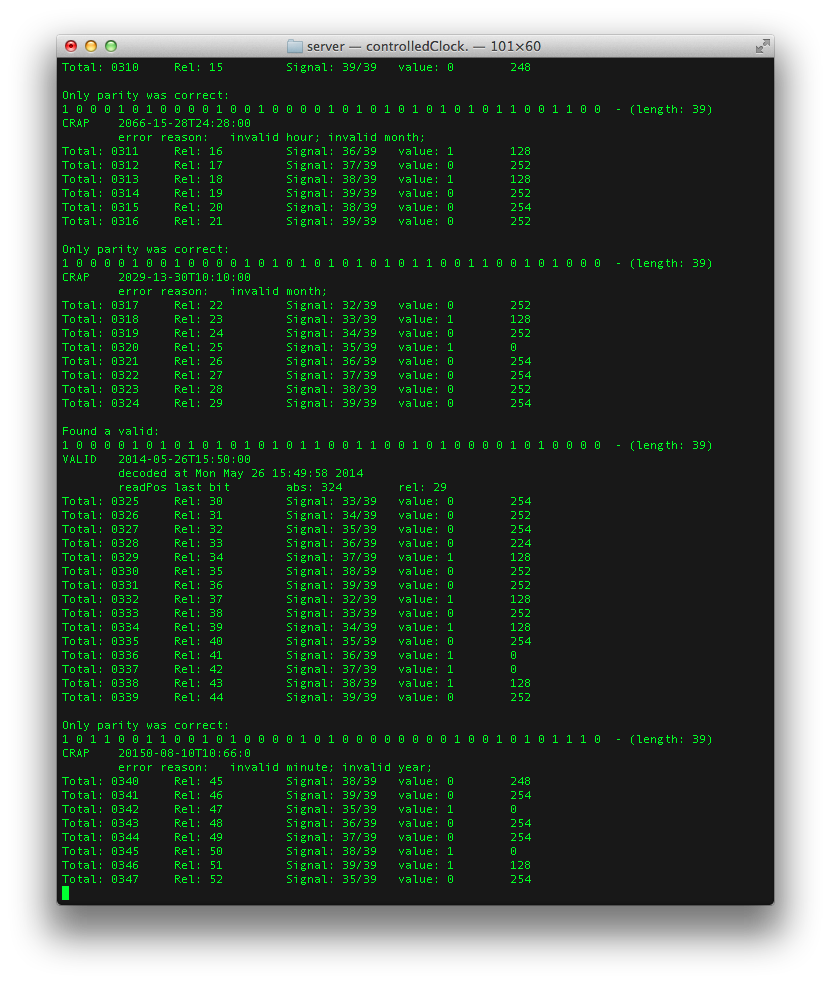
\includegraphics[width=0.8\textwidth]{./images/screenshots/server_console_output.png}
\end{figure}

\begin{figure}[htbp!]
	% \vspace{-20pt}
	\caption{HTTP Request auf Webserver}
	\centering
		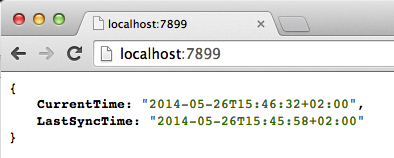
\includegraphics[width=0.5\textwidth]{./images/screenshots/server_webresponse.png}
\end{figure}

\newpage

\subsection{Client}
\begin{figure}[htbp!]
	\caption{Client nach Aufruf (vollständig geladen und initialisiert)}
	\centering
		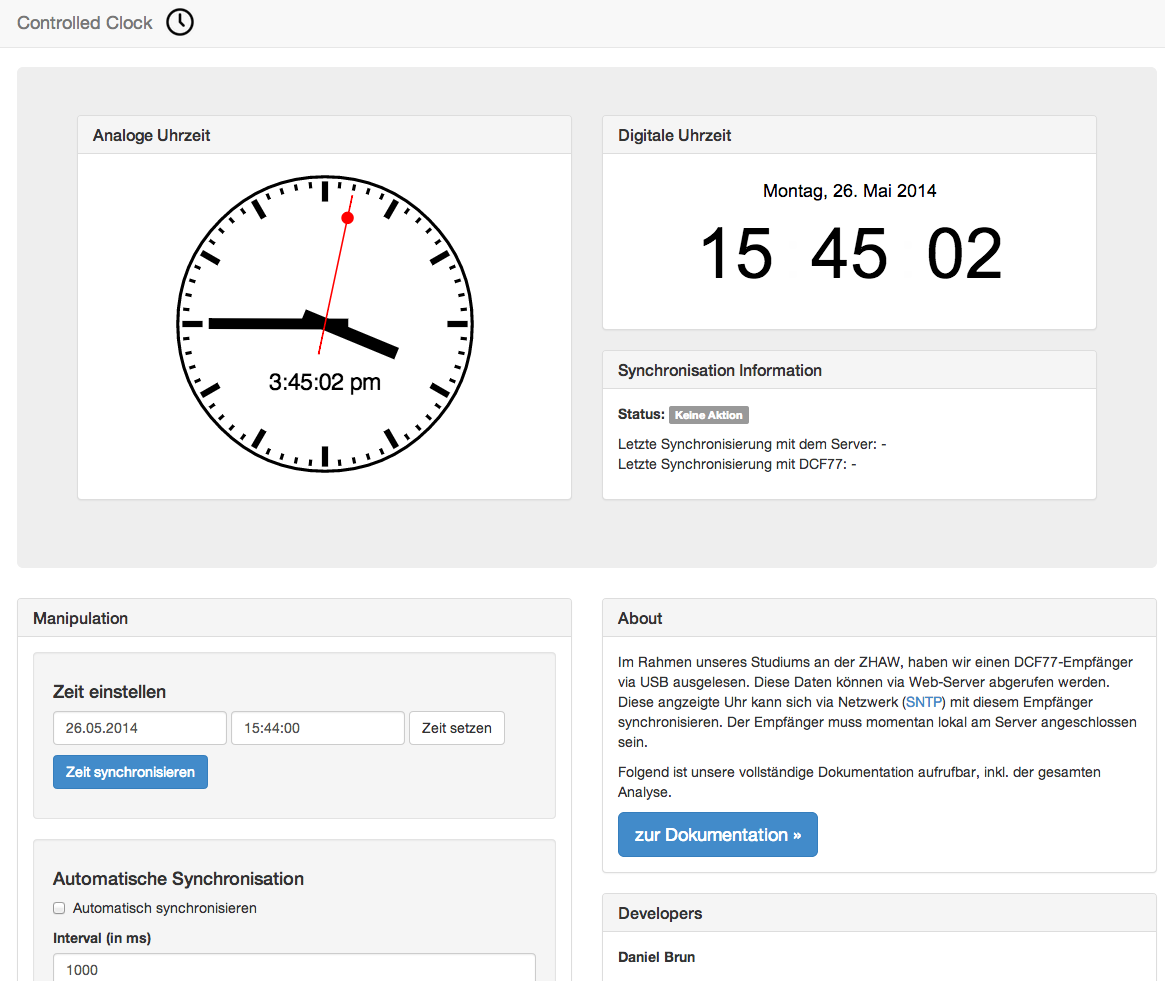
\includegraphics[width=0.9\textwidth]{./images/screenshots/client_full_initialised.png}
\end{figure}

\begin{figure}[htbp!]
	\caption{Eintstellmöglichkeiten via Web-GUI}
	\centering
		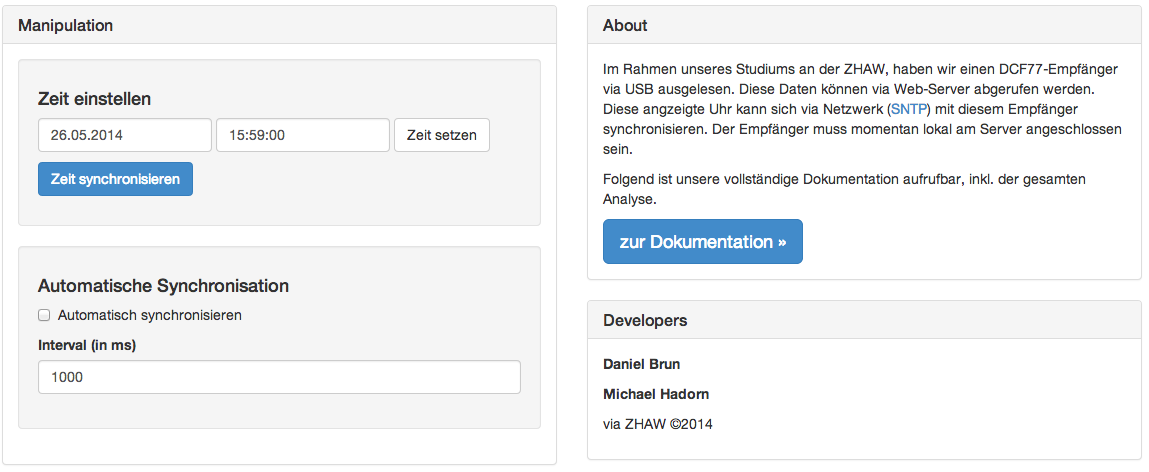
\includegraphics[width=0.9\textwidth]{./images/screenshots/client_controlling.png}
\end{figure}

\begin{figure}[htbp!]
	\caption{Synchronisation ohne DCF77 Signal}
	\centering
		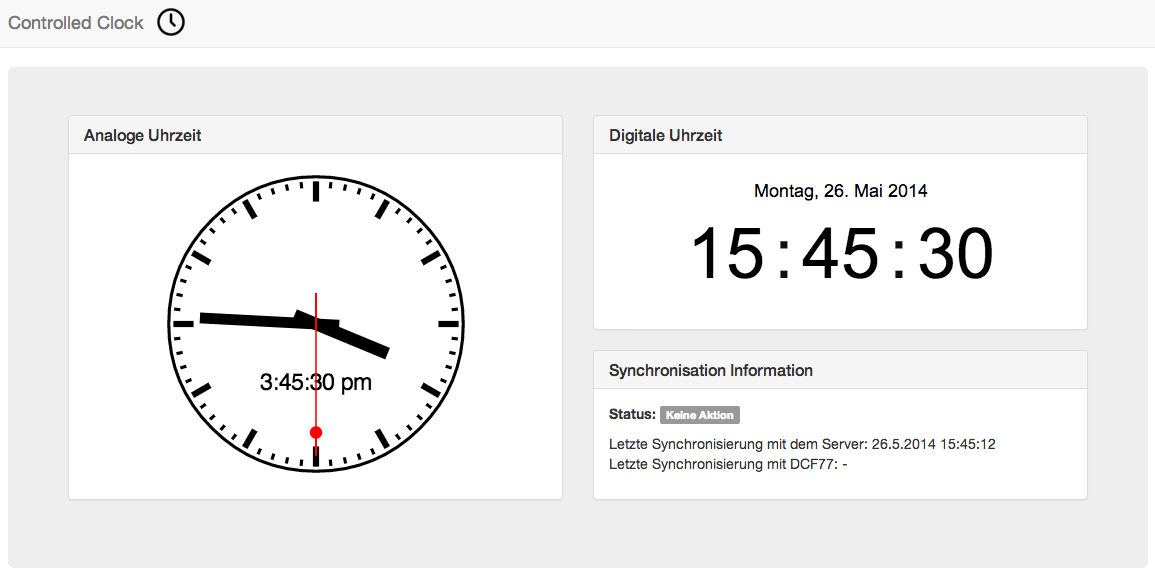
\includegraphics[width=1\textwidth]{./images/screenshots/client_clock_sync_without_dcf77.png}
\end{figure}

\begin{figure}[htbp!]
	\caption{Synchronisation mit gültigem DCF77 Signal}
	\centering
		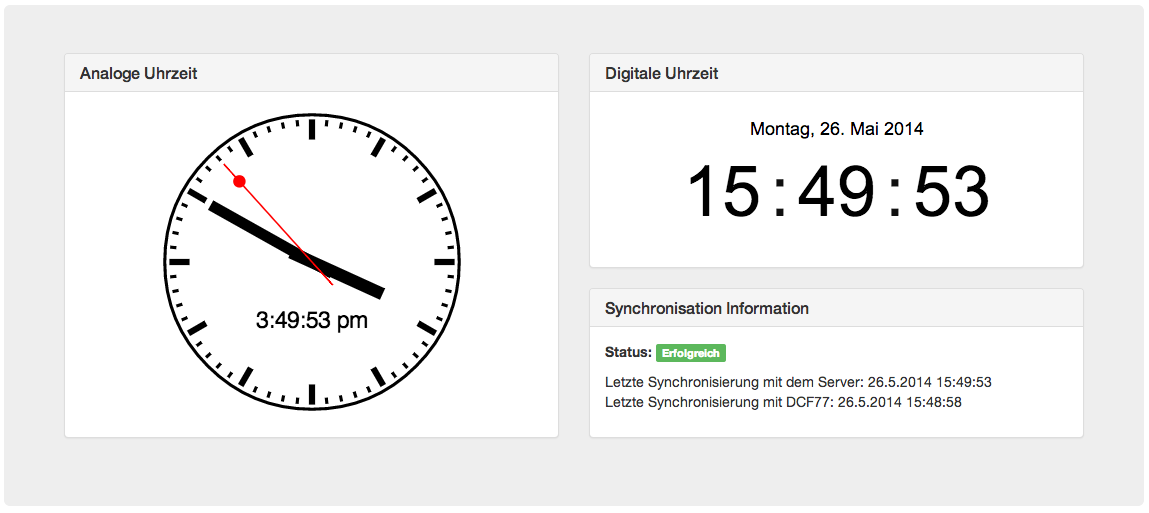
\includegraphics[width=1\textwidth]{./images/screenshots/client_clock_sync_with_dcf77.png}
\end{figure}